\documentclass{article}
\usepackage{tikz}
\usepackage{relsize}
\usetikzlibrary{automata, positioning, arrows, fit, shapes}
\usepackage{amsmath}

\begin{document}

\title{NFA State Diagram for Language B (General Case)}

\author{COMP 382 Assignment 1}
\date{{\fontsize{8}{9.6}\selectfont Ryan Austin, Prasoon Tyagi}} % Smaller date (8pt)

\maketitle

\section{General Construction for Arbitrary Even k}

For an arbitrary even constant $k$ where $k \geq 2$, we construct an NFA as follows:

\subsection{Examples given $k$ = 4}
For $k=4$, we read the first 4 positions and append the characters at even positions ($w_2$ and $w_4$).
\begin{itemize}
    \item $w = 0111 \Rightarrow 0111 \cdot 11 = 011111$ (positions $w_2$,$w_4$ are both 1, append "11")
    \item $w = 1000 \Rightarrow 1000 \cdot 00 = 100000$ (positions $w_2$,$w_4$ are both 0, append "00")
    \item $w = 1100 \Rightarrow 1100 \cdot 10 = 110010$ (position $w_2$ is 1, position $w_4$ is 0, append "10")
\end{itemize}

\subsection{State Diagram for arbitrary $k$}

\begin{center}
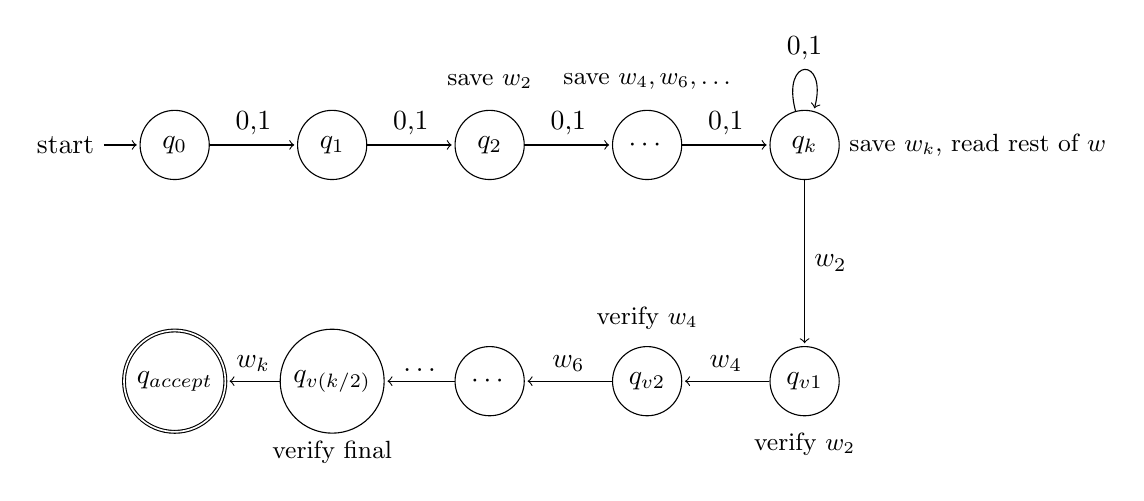
\begin{tikzpicture}[shorten >=1pt, node distance=2cm, on grid, auto]
   % Reading phase
   \node[state, initial] (q0) {$q_0$};
   \node[state] (q1) [right=of q0] {$q_1$};
   \node[state] (q2) [right=of q1] {$q_2$};
   \node[state] (qdots1) [right=of q2] {$\cdots$};
   \node[state] (qk) [right=of qdots1] {$q_k$};
   
   % Verification phase
   \node[state] (qv1) [below=3cm of qk] {$q_{v1}$};
   \node[state] (qv2) [left=of qv1] {$q_{v2}$};
   \node[state] (qvdots) [left=of qv2] {$\cdots$};
   \node[state] (qvkover2) [left=of qvdots] {$q_{v(k/2)}$};
   \node[state, accepting] (qacc) [left=of qvkover2] {$q_{accept}$};
   
   % Annotations
   \node[above=0.8cm of q2, text=black, font=\small] {save $w_2$};
   \node[above=0.8cm of qdots1, text=black, font=\small] {save $w_4, w_6, \ldots$};
   \node[right=2.2cm of qk, text=black, font=\small] {save $w_k$, read rest of $w$};
   
   \node[below=0.8cm of qv1, text=black, font=\small] {verify $w_2$};
   \node[above=0.8cm of qv2, text=black, font=\small] {verify $w_4$};
   \node[below=0.9cm of qvkover2, text=black, font=\small] {verify final};
   
   % Reading phase transitions
   \path[->]
   (q0) edge node {0,1} (q1)
   (q1) edge node {0,1} (q2)
   (q2) edge node {0,1} (qdots1)
   (qdots1) edge node {0,1} (qk)
   (qk) edge[loop above] node {0,1} (qk);
   
   % Branching to verification
   \draw[->] (qk) -- node[right] {$w_2$} (qv1);
   
   % Verification phase transitions
   \path[->]
   (qv1) edge node[above] {$w_4$} (qv2)
   (qv2) edge node[above] {$w_6$} (qvdots)
   (qvdots) edge node[above] {$\ldots$} (qvkover2)
   (qvkover2) edge node[above] {$w_k$} (qacc);
   
\end{tikzpicture}
\end{center}
\newpage

\subsection{Formal Definition}

The NFA $M$ for language $B$ is formally defined as a 5-tuple $M = (Q, \Sigma, \delta, q_0, F)$ where:

\begin{itemize}
    \item $Q$: Finite set of states including reading states $\{q_0, q_1, \ldots, q_k\}$, verification states $\{q_{v1}, q_{v2}, \ldots, q_{v(k/2)}\}$, and accept state $q_{accept}$
    \item $\Sigma = \{0, 1\}$: The binary alphabet
    \item $\delta: Q \times \Sigma \to 2^Q$: The transition function (mapping to power set of $Q$ for nondeterminism)
    \item $q_0 \in Q$: The start state
    \item $F = \{q_{accept}\}$: The set of accept states
\end{itemize}

\section{Explanation}
\noindent\textbf{Model Clarification:}
The described automaton is a nondeterministic finite automaton (NFA). 
At each even position $i \in \{2,4,\ldots,k\}$, the value of $w_i$ is encoded 
into the current state. Transitions labeled $w_i$ represent transitions on either $0$ or $1$, 
depending on the value stored in the state. 
Since $k$ is a fixed constant, the total number of such states is finite.
\\\\
Since there are $k/2$ even positions and each can take one of two binary values, 
there are $2^{k/2}$ possible combinations of $(w_2, w_4, \ldots, w_k)$, each of which 
can be encoded into a distinct state of the automaton.
\\\\
\noindent\textbf{Reading Phase (states $q_0$ through $q_k$):}
\begin{itemize}
    \item The states $q_0, q_1, \ldots, q_k$ read the first $k$ characters of the input
    \item At each even position $i \in \{2, 4, 6, \ldots, k\}$, we remember the character $w_i$
    \item The state $q_k$ has a self-loop to continue reading characters beyond position $k$ (for strings where $n \geq k$)
\end{itemize}

\noindent\textbf{Verification Phase (states $q_{v1}$ through $q_{v(k/2)}$):}
\begin{itemize}
    \item From $q_k$, we non-deterministically branch to $q_{v1}$ when we read a character matching $w_2$
    \item State $q_{v1}$ verifies the first suffix character matches $w_2$
    \item State $q_{v2}$ verifies the next character matches $w_4$
    \item Continue sequentially through verification states
    \item State $q_{v(k/2)}$ verifies the final suffix character matches $w_k$
    \item If all verifications succeed, transition to $q_{acc}$ (accept state)
\end{itemize}

\newpage

\section{Design Choices and Justification}

\subsection{Why NFA over DFA?}
We chose to construct a nondeterministic finite automaton (NFA) rather than a deterministic finite automaton (DFA) because:
\begin{itemize}
    \item The NFA construction is more intuitive - we non-deterministically guess when the suffix begins
    \item An equivalent DFA would require exponentially many states ($2^{k/2}$ combinations) to track all possible values of remembered characters
    \item NFAs are equivalent to DFAs in computational power, so proving regularity with an NFA is sufficient
\end{itemize}

\subsection{State Diagram Design}
We structured the diagram in two phases (reading and verification) to clearly show:
\begin{itemize}
    \item The separation between reading the main string and verifying the suffix
    \item The self-loop at $q_k$ handles strings of arbitrary length $n \geq k$
    \item Annotations help visualize which characters are stored at each step
\end{itemize}

\subsection{Implementation Approach}
Our Python implementation simulates the NFA by:
\begin{itemize}
    \item Splitting the input into main string and suffix
    \item Extracting characters at even positions from the main string
    \item Comparing the suffix to the extracted characters
    \item This direct approach is simpler than tracking all possible NFA states
\end{itemize}

\section{Conclusion}
Since $k$ is a \emph{constant}, the number of states is \emph{finite}, regardless of the input length $n$. We can construct an NFA with finitely many states that recognizes language $B$. Since every NFA recognizes a regular language, we conclude that $B$ is regular. Therefore, language $B$ is regular for any even constant $k$. \qed

\newpage

\begin{thebibliography}{2}

\bibitem{sipser2013}
Sipser, Michael. 
\textit{Introduction to the Theory of Computation}. 
3rd ed., 2013.

\bibitem{rabin1959}
Rabin, Michael O., and Dana Scott. 
``Finite Automata and Their Decision Problems.'' 
\textit{IBM Journal of Research and Development}, vol. 3, no. 2, 1959, pp. 114-125.

\bibitem{hopcroft2006}
Hopcroft, John E., Rajeev Motwani, and Jeffrey D. Ullman. 
\textit{Introduction to Automata Theory, Languages, and Computation}. 
3rd ed., Pearson, 2006.

\bibitem{courselectures}
``COMP 382: Languages, Computations and Machines.'' 
Course Lecture Notes, University of the Fraser Valley, 2026.

\bibitem{claude}
Anthropic. 
``Claude AI Assistant.'' 
\textit{Claude.ai}, 2026, claude.ai. 
Used for debugging NFA transition logic, researching and LaTeX formatting.

\bibitem{copilot}
Microsoft and OpenAI. 
``GitHub Copilot.'' 
\textit{GitHub.com}, 2026, github.com/features/copilot. 
Used for code completion and debugging assistance in Visual Studio Code.

\end{thebibliography}

\end{document}